%====================================================================================================
% ?????
%====================================================================================================
% TCC
%----------------------------------------------------------------------------------------------------
% Autor				: Jasane Schio
% Orientador		: Gedson Faria
% Co-Orientador		: Angelo Darcy
% Instituição 		: UFMS - Universidade Federal do Mato Grosso do Sul
% Departamento		: CPCX - Sistema de Informação
%----------------------------------------------------------------------------------------------------
% Data de criação	: 01 de Outubro de 2015
%====================================================================================================
% Define o caminho das figuras
\graphicspath{{figuras/}}
\chapter{Fundamentação Teórica} \label{Cap:Fundamentacao}
\section{Considerações Iniciais}
Neste capítulo serão abordados os temas relacionados as imagens digitais, o universo de cores e o futebol de robôs. Incia-se com as teorias sobre o processamento digital de imagens, detecção de objetos e detecção de bordas. Apresenta-se também os estudos sobre as Cores, explicando seus espaços, sistemas e modelos de cores. Por fim, descreve-se o ambiente do futebol de robôs e as regras para categoria VSSS.

%Como designado na seção 1.4 deste trabalho, estudou-se dentro da área de processamento de imagens a detecção de objetos que por sua vez se faz possível utilizando a técnica de detecção de bordas.

\section{Processamento Digital de Imagens}

O processamento digital de imagens é uma área de estudo que consiste na manipulação da imagem e seus elementos, transformando-a visando obter mais facilmente as informações nela contidas\cite{Albuquerque:2001}. Além da retirada de informações, o processamento de imagens também inclui a modificação ou melhoria da imagem por meio de redução de ruídos, melhoria no contraste, segmentações da imagem entre outras técnicas.
\citeonline{Gonzalez:2008} escrevem que embora não existam barreiras definidas, um imagem pode ser processada de três maneiras: 
\begin{description}
	\item[Processo de baixo nível] aplica ações primitivas de modificação de imagem. Este processo tem como caraterística seu resultado final ser também uma imagem, semelhante a imagem inicial contendo melhorias.
	\item[Processo de nível intermediário] consiste na divisão de uma imagem em regiões ou objetos, afim de processa-los individualmente para obter suas informações. Se carateriza por seu resultado final ser muitas vezes apenas regiões, objetos ou outras informações extraídas da imagem.
	\item[Processo de alto nível] se define por ser um processamento mais sensorial. Trata-se da análise de objetos usando funções cognitivas associadas a visão computacional, essa usa informações relevantes para o reconhecimento de objetos.
\end{description}
% Dentre os tipos de processamento de imagens existe, \citeonline{Gonzalez:2008} os define como: aplicações de ações primitivas de modificação de imagem, esta caraterizada por seu resultado final ser também uma imagem semelhante a imagem inicial porém modificada(Low-Level-Process), divisão de imagem em regiões e alguns tipos de reconhecimento e classificação de objetos, caraterizada por seu resultado final ser muitas vezes apenas regiões ou informações da imagem inicial(Mid-Level-Process), e o mais sensorial de todos que é a analise de objetos usando funções cognitivas associadas a visão computacional, essa usa informações relevantes para o reconhecimento de objetos(Higher-Level-Process). 
%Uma vez que o objetivo deste trabalho é reconhecer os objetos em campo para calibra-los, usaremos técnicas de retirada de  objetos juntamente com técnicas de análise de informações, processamento de nível intermediário e alto.

\subsection{Detecção de Objetos}
\label{Sec:TiposDeDeteccaoDeObjetos}
%Antes de descrever os métodos de classificação devemos fazer algumas definições:
%\begin{itemize}
%	\item	Em cada detecção de objetos são obtidas as informações sobre a imagem, essas são de acordo com o tipo de detecção desejada. Os dados podem conter informações como posição, tamanho, borda, transformação linear, rotação entre outros. Cada detecção em uma imagem é chamada de pose.
	
%	\item	Métodos de detecção de objeto baseado em classes constroem a classe do objeto baseada em um conjunto de treino. O conjunto de treino é composto por múltiplas imagens exemplo do objeto para que seja assim capturado os aspectos do objeto.
%\end{itemize}

A detecção de objetos é uma das áreas de visão computacional que obtêm muita atenção dos pesquisadores, contudo, pode ser considerada uma técnica herdada do reconhecimento de padrões, pois consiste em separar objetos por categorias de acordo com uma ou mais características específicas. Ou seja, devido a junção das técnicas de reconhecimento de padrões com o processamento digital de imagens tornou-se possível a detecção de objetos em imagens\cite{Nascimento:2007}.

O primeiro {\it framework} de métodos que usam base de dados categorizando uma ou mais características de um objetos para fazer o reconhecimento por meio de aprendizado foi apresentado por \citeonline{Viola:2001}. Desde o {\it framework} de Viola e Jones até os dias atuais, muitos métodos e teorias para detecção já foram propostos e implementados, como detecção de faces utilizando um classificador de redes neurais na intensidade de padrões de uma imagem \cite{Rowley:1998, Garcia:2004}, {\it support vector machine} para localizar rostos humanos e carros \cite{Osuna:1997, Papageprgiou:1999}, análise de componentes principais \cite{Jolliffe:2002}, análise independente de componentes\cite{Hyvarinen:2004}, fatoração de matriz não-negativa \cite{Lee:1999} , análise discriminativa linear \cite{Duda2012},  {\it boosting} \cite{Freund:1995}, classificação binária, que considera a detecção do objeto em tamanho fixo apenas variando a posição na imagem \cite{AmitFelzenszwalb:2014}, além de algoritmos de análise estrutural topológica por {\it border-following} \cite{Suzuki:1985} que é utilizado na bibliotecas de processamento digital de imagens OpenCV \cite{OpenCV}.

%Em 2005 Ulusoy e Bishop\cite{Ulusoy:2005} mostraram o quão útil seria categorizar os métodos de detecção de imagens, e os dividiram em duas principais categorias: generativa e discriminativa. Categorias que foram aceitas e utilizadas como mostram Amit e Falzenszwalb\cite{AmitFelzenszwalb:2014} e Roth e Winter\cite{Roth:2008}.

%O método generativo pode ser descrito como um modelo probabilístico para a variância da pose de um objeto juntando com o modelo de aparência, ou seja, um modelo de probabilidade para a aparência da imagem condicional em uma determinada pose, juntamento com um modelo de fundo. Os parâmetros do modelo são estimados a partir de dados retirados de treinamento e as decisões são baseadas nas probabilidades anteriores\cite{AmitFelzenszwalb:2014}. Em resumo o método generativo tenta encontrar uma representação adequada dos dados originais através da aproximação dos dados originais, mas mantendo o máximo de informação possível\cite{Roth:2008}.

%Já o modelo discriminativo tipicamente constrói um classificador que pode discriminar entre imagens (ou sub-imagens) contendo o objeto e as que não contém o objeto. Os parâmetros do classifidor são selecionados para minimizar os erros nos dados de treino\cite{AmitFelzenszwalb:2014}.


%	Ulusoy\cite{Ulusoy:2005} apontou as principais vantagens dos dois metodos. 
%Segundo Ulusoy e Bishop\cite{Ulusoy:2005} o método generativo se destaca por tratar perda de dados ou dados parcialmente rotulados, pela facilidade em que uma nova classe pode ser incrementada na classificação condicional de densidade, independentemente das classes anteriores, e por conseguir facilmente lidar com composição de objetos (ex: óculos, chapéus...), considerando que os modelos discriminativos precisar analisar todas as combinações durante o treinamento. Amit e Felzenszwalb\cite{AmitFelzenszwalb:2014} ainda aponta que as vantagens descritas sobre o método discriminativo são ditas como a flexibilidade do modelo  que pode ser utilizado em regiões do espaço de entrada onde as probabilidades posteriores diferem significativamente de 0 ou 1, ao passo que as abordagens detalhes generativas modelo de distribuição de X, que podem ser irrelevantes para determinar as probabilidades posteriores, além de ser tipicamente muito rápido em fazer previsões para os novos pontos (teste) de dados, enquanto os modelos generativos muitas vezes exigem solução iterativa, e pela igualdade de circunstâncias, seria de esperar que os métodos discriminativos tenham melhor desempenho preditivo, uma vez que são treinados para prever o rótulo de classe em vez de a distribuição conjunta de vetores e alvos de entrada.

\subsection{Detecção de Bordas}
Para um objeto poder ser destacado por algum método de detecção, a imagem passa por um processo de segmentação. A segmentação pode ser dita como o processo de divisão da imagem em objetos\cite{Gonzalez:2008}. De acordo com \citeonline{Wangenheim:2014}, o processo de segmentação se baseia em dois conceitos: similaridade e descontinuidade. A descontinuidade é o processo no qual se separa o fundo das partes e estas umas das outras, utilizando-se linhas, bordas ou pontos. Já a similaridade é o processo no qual os pixeis provenientes da descontinuidade são agrupados de acordo com a proximidade um dos outros para formar os objetos de interesse. 

De acordo com \citeonline{Canny:1986}, a detecção de bordas é um processo simplificado que serve para diminuir drasticamente o total de dados a serem processados e ao mesmo tempo preservar informações valiosas sobre os objetos. %este também é considerado um processamento de imagem de baixo nível, uma vez que age diretamente na imagem original melhorando-a. É muito comum a ocorrência de ruídos quando se trata da detecção de bordas, e por sua vez para evitar esses ruídos é necessário a suavização da imagem antes de fazer a detecção. 
%\citeonline{Vale:2002} lembra que a suavização possui pontos negativos como perda de informação e deslocamento de estruturas de feições proeminentes no plano da imagem. Além disso, existem diferenças entre as propriedades dos operadores diferenciais comumente utilizados, o que ocasiona  bordas diferentes. 
Assim, como dito por \apudonline{Ziou1998}{Vale:2002}, se torna difícil encontrar um algoritmo que tenha bom desempenho em diferenciados contextos e capture os requisitos necessários aos estágios subsequentes do processamento. 
Quando se trata de detecção de bordas existem dois critérios que devem ser levados em consideração, Taxa de Erro e Localização \cite{Canny:1986, Vale:2002}. 

\begin{description}
	\item[Taxa de Erro] É importante que as bordam contidas na imagem não sejam confundidas ou perdidas, tampouco que não sejam detectadas bordas falsas. É necessário que o algoritmo de detecção de borda tenha uma baixa taxa de erro para que seja eficiente \cite{Wangenheim:2014, Canny:1986, Vale:2002}.
	\item[Localização] A distância entre os pixeis de borda encontradas pelo algoritmo e a borda atual deveriam ser o menor possível \cite{Wangenheim:2014}.
\end{description}
Ao tentar aplicar esses dois critérios para desenvolver um modelo matemático para detecção de bordas, sem a necessidade de base em regras preestabelecidas, no artigo 
\textit{A Computational Approach to Edge Detection}, \citeonline{Canny:1986} descreve que somente esses dois critérios não são suficientes para obter uma boa precisão da detecção de bordas, portanto, propôs um terceiro critério: Resposta.
\begin{description}
	\item[Resposta] Para contornar a possibilidade de mais de uma resposta para a mesma borda, ou seja, o detector de bordas não deveria identificar múltiplos pixeis de borda onde somente exista um único pixel.
\end{description}

Com o acréscimo do terceiro critério, o processo de detecção de bordas de \citeonline{Canny:1986}
mostrou-se bastante flexível, independente da origem da imagem utilizada\cite{Vale:2002}.

 \begin{figure}[H]
	\centering
	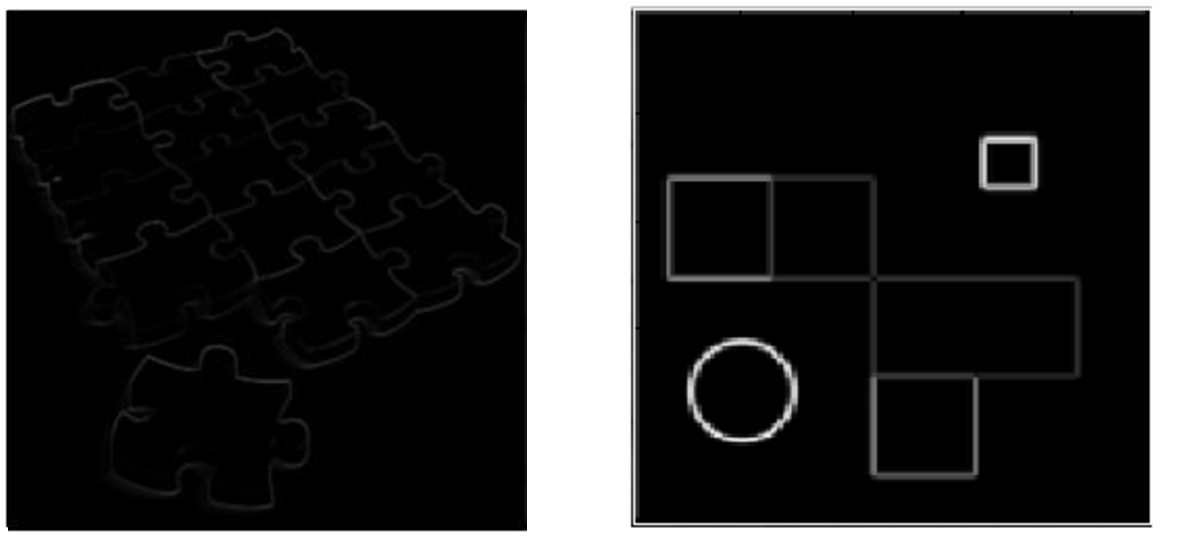
\includegraphics[width=0.8\textwidth]{canny.pdf}
	\caption{Detecção de Borda com Algoritmo de Canny\cite{Saini:2013} }
	\label{Canny}
\end{figure}







\section{Universo de Cores} \label{Sec:Cores}

Para redação desta seção foi tomada como base o Capítulo 5, Cores, de \citeonline[pp. 181-212]{Azevedo:2003}.

O olho humano é capaz de identificar cores mesmo com as mais diferentes interferências, luminosidade, tonalidade, intensidade, entre outras ações de agentes externos, graças aos \textbf{cones} e \textbf{bastonetes}. Os bastonetes são os responsáveis por distinguirem tons de cinza e pela visão periférica e tem como característica serem sensíveis a baixo nível de luminosidade, os cones, como descrito por \citeonline{Azevedo:2003}, ``são sensíveis ao alto nível de iluminação e responsáveis pela percepção de cores". Segundo a teoria tricomática de Thomas Young, aprimorada por Hermann von Helmholtz, a retina humana é formada por três tipos de fotopigmentos que seriam os três receptores de cor, ou seja, respondiam ao comprimento de onda de apenas três cores: Vermelho, Verde e Azul \cite{Azevedo:2003}. 

A informação obtida pelo sistema visual humano é assimilada pelo cérebro, ligando a cor a sua aparência, levando em consideração o aprendizado que obtivemos sobre a mesma. Já para uma máquina, cores são representadas como números, na qual cada cor contém um código específico. Para o nosso cérebro é muito fácil entender, por exemplo, que as cores verde, verde lima e verde escuro são parte da mesma cor: verde, apenas possuem tonalidades diferentes. Para o computador cada uma das tonalidades é representada por um código diferente, e cada nível de luminosidade nessas cores, as modificam, tornando-se códigos diferentes das cores originais.


Quando fez sua primeira experiência com a decomposição da luz em um prisma para obter cores Newton percebeu que não havia a cor branca. Ele tentou então misturar as sete cores que obteve para gerar a branca, porém, não obteve sucesso.
A resposta para o porque de Newton não ter conseguido chegar à cor branco veio somente em 1931, quando a Comissão Internacional de Iluminação(CEI) definiu três primarias (X, Y e Z) que combinadas formam todas as cores e que existe duas formas de se obter cores: através da emissão ou reflexão de luz \cite{Souto:2003}. Assim, entendeu-se o porque em seu experimento Newton não ter sucesso. Para gerar a cor branca é necessário a soma das três cores primarias azul, verde e vermelho, uma vez que seu experimento utilizava a reflexão e não emissão de cores.
Estas formas de se obter cores são conhecidas como \textbf{Sistemas de cores}. O sistema de cor relativo a emissão de luz é o RGB e o sistema de reflexão de luz é conhecido como CMY, ambos são mostrados na Figura \ref{fig:sistemasdecores}.
 \begin{figure}[H]
 	\centering
 	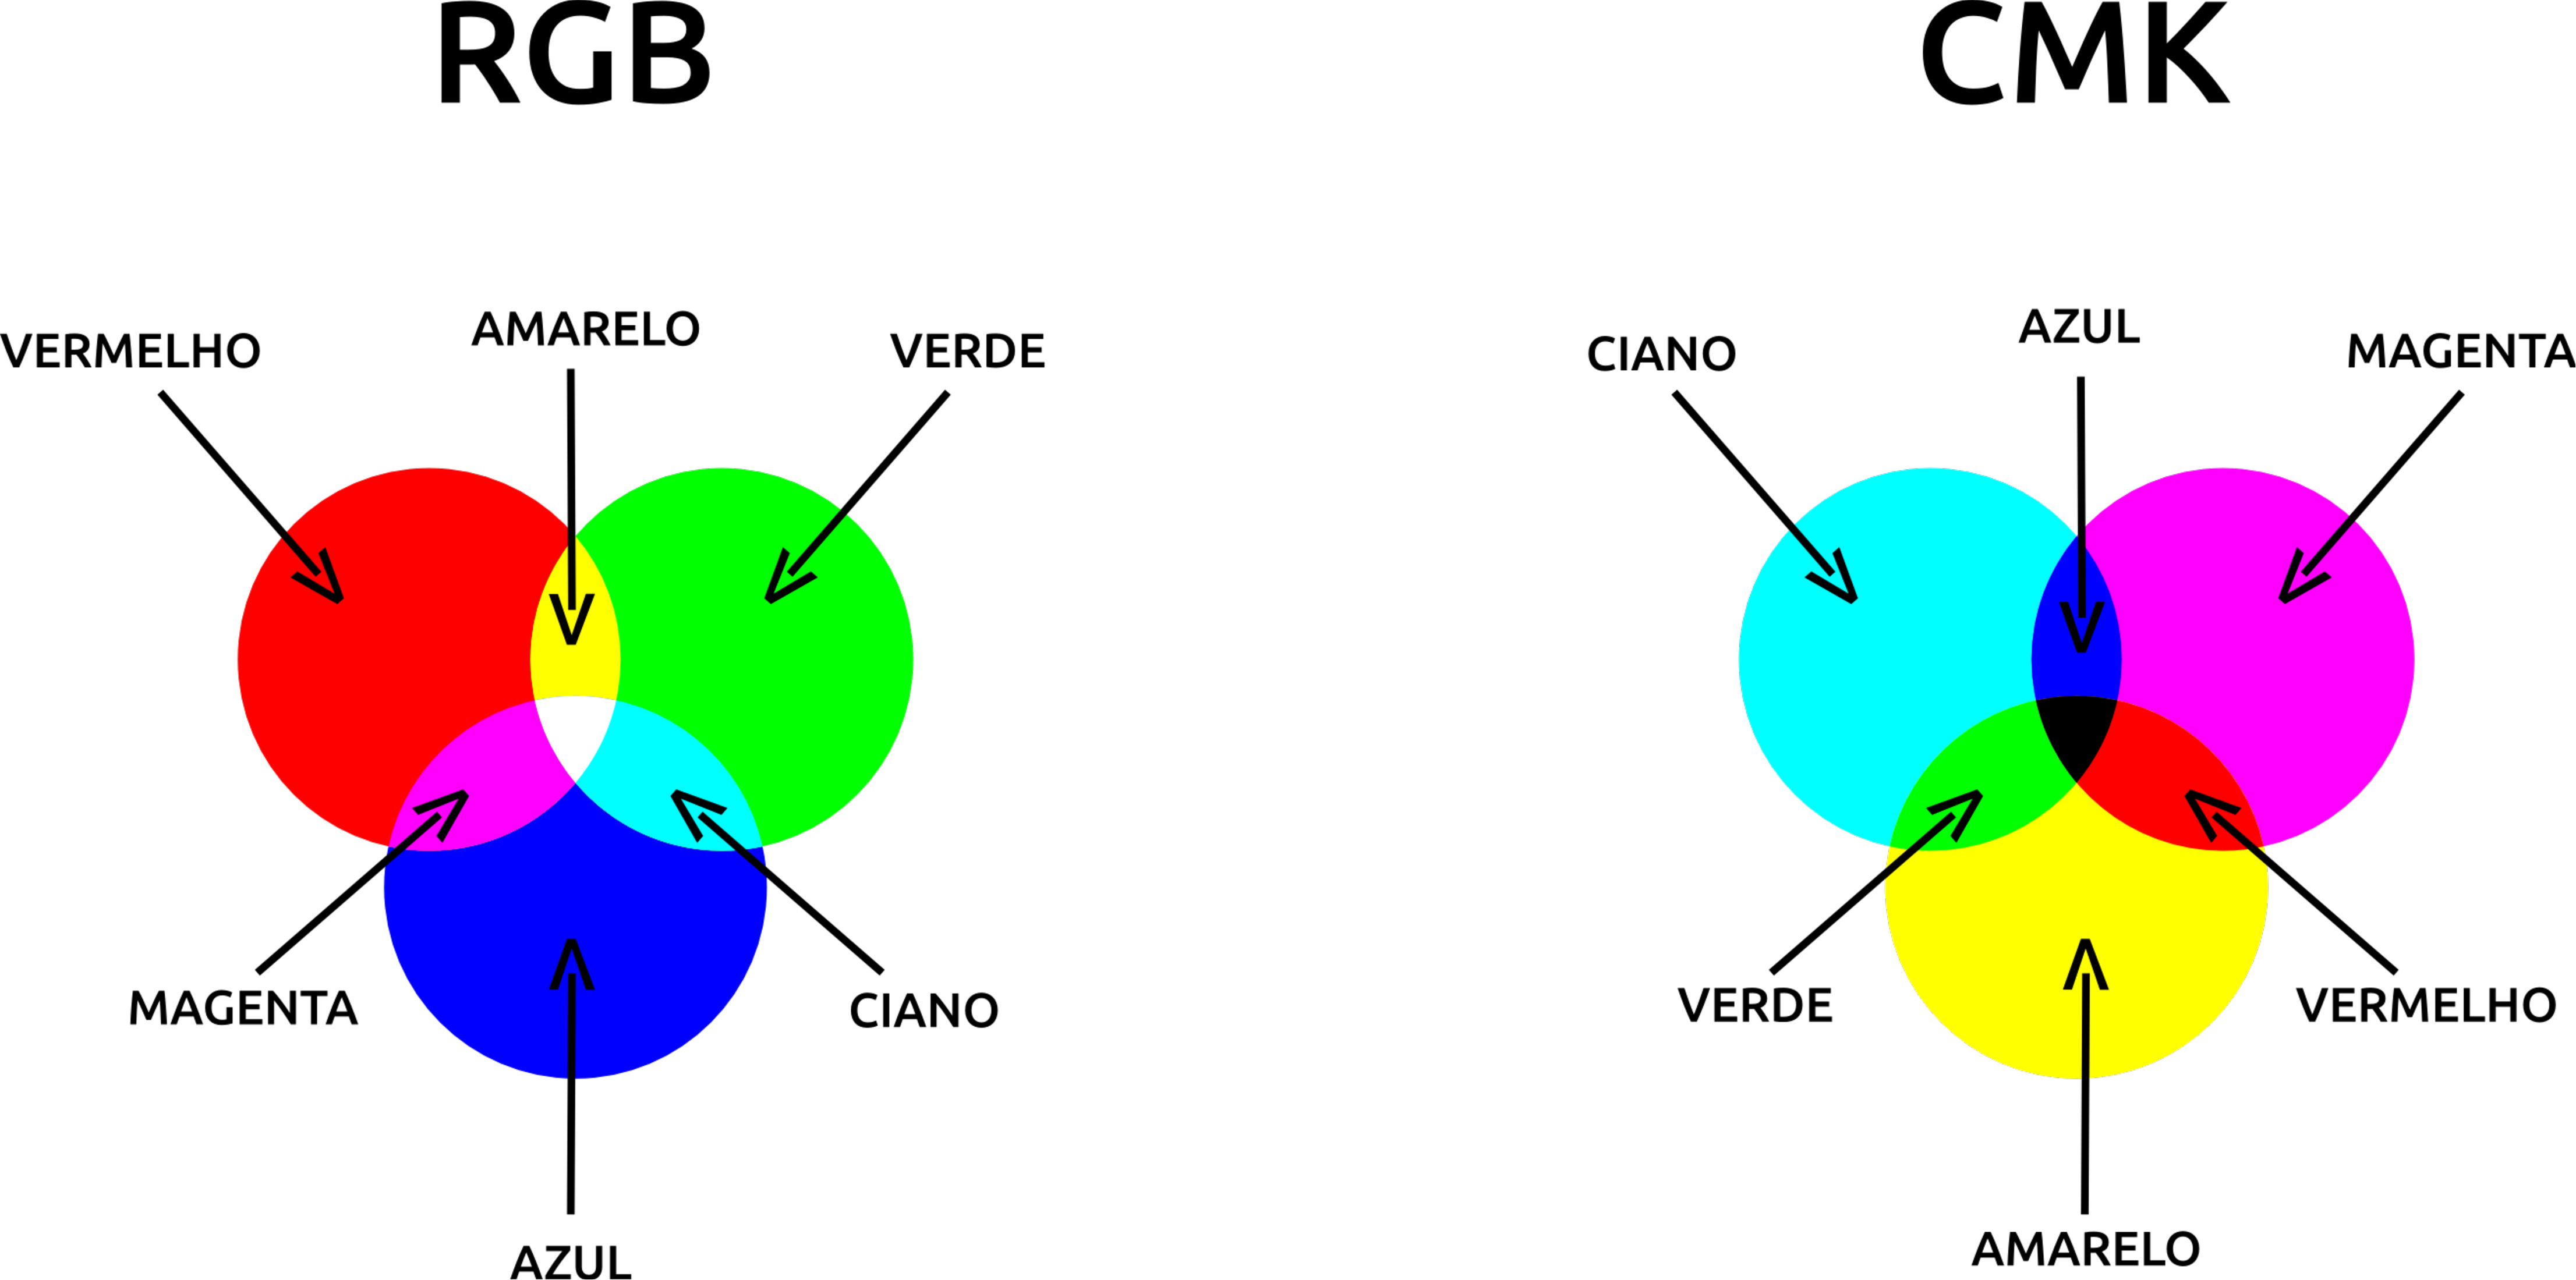
\includegraphics[width=0.5\textwidth]{espacos.pdf}
 	\caption{Exemplo dos sistemas de cores RGB E CMY.}
 	\label{fig:sistemasdecores}
 \end{figure}

Juntamente com a definição dos sistemas de cor, foi proposto o Diagrama de cromaticidade, exposto na Figura \ref{fig:DiagramadeCores}, representando as cores presentes no espectro da luz visível \cite{Souto:2003}, ou seja, todas as cores puras visíveis . O diagrama é apresentado por uma forma plana contendo somente a cromaticidade das cores, luminosidade e intensidade são consideradas em um ponto invariável.
 
 
 \begin{figure}[H]
 	\centering
 	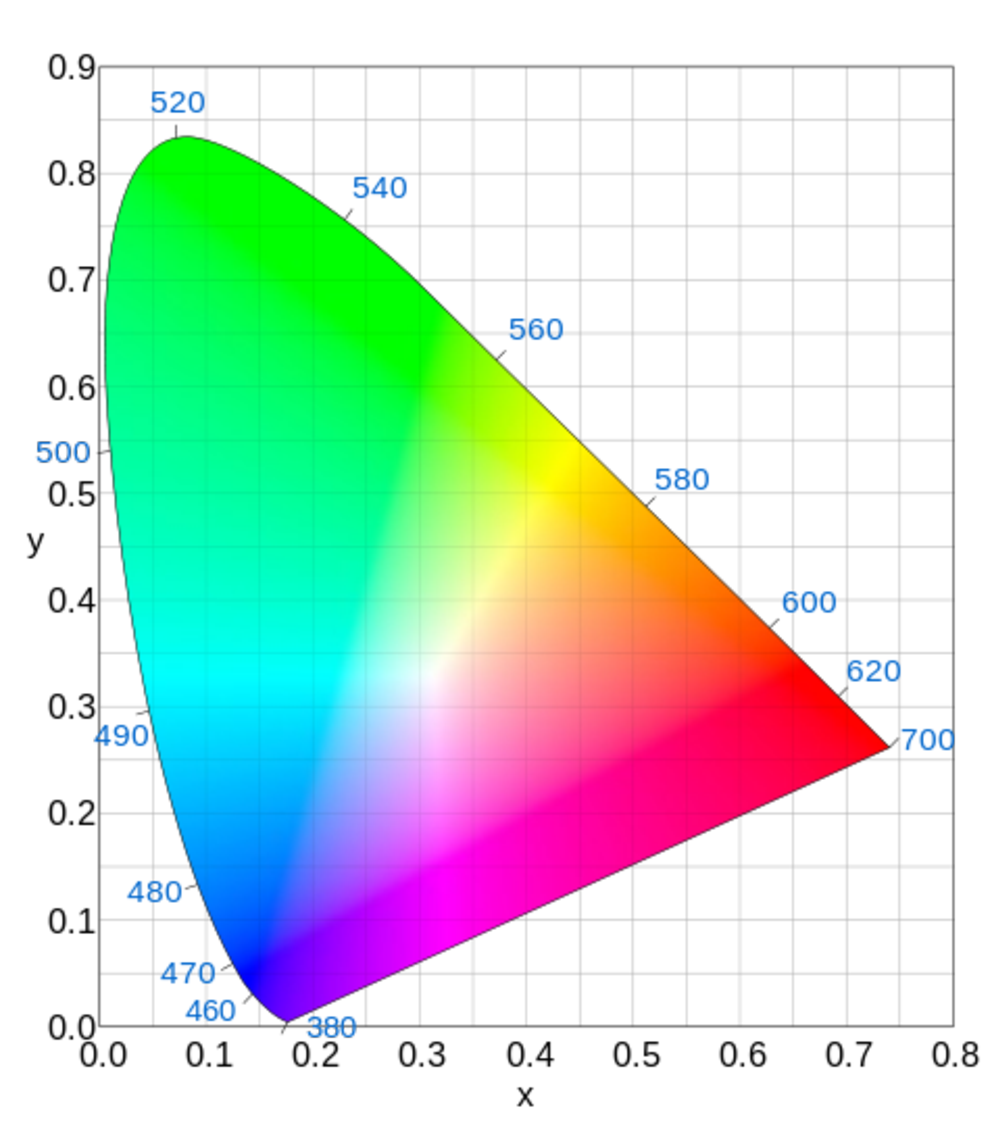
\includegraphics[width=0.25\textwidth]{graficocie.pdf}
 	\caption{Diagrama de cromaticidade estabelecido pelo CIE.}
 	\label{fig:DiagramadeCores}
 \end{figure}

Segundo \citeonline{Azevedo:2003} as cores que podem ser reproduzidas por um sistema cores é chamado de \textbf{Espaço de Cores}. \apudonline{Foley:2013}{Souto:2003} define o espaço de cores como sendo tridimensional com coordenadas correspondentes a cada uma das cores primárias. O valor do eixo é designado pela quantidade necessária de cor primária na reprodução de uma determinada cor. O espaço de cores pode ser entendido como a quantidade de detalhamento, tonalidades de uma cor, dentro do espectro de cores de um determinado modelo de cor.

Para utilização das teorias de sistemas e espaços de cores, foram criados os \textbf{Modelos de Cores} para descrever as cores na prática. Neste trabalho, será dado enfoque  nos modelos RGB e HSV, devido a sua relevância na utilização da biblioteca OpenCV.

Modelo de cores são modelos matemáticos utilizados para classificação das cores de acordo com sua tonalidade, saturação, luminosidade ou crominância na tentativa de conseguir cobrir o maior número de cores possíveis e assim simulando a visão. A representação da cor é definida por um único ponto em um modelo tridimensional. 
Os modelo de cores tem como função definir as cores nos programas gráficos de computadores, de forma que combine com a 
percepção das cores pelo sistema visual humano que também utiliza três eixos similares para definição da cor \cite{Leao:2005}.

O modelo de cores RGB pode ser considerado mais básico dos modelos de cores. Seu nome possui a mesma definição do espaço de cores RGB, e não utiliza  atributos como luminosidade ou tonalidade, criando-se cores pela combinação das cores primárias azul, verde e vermelho (Figura \ref{fig:ModeloRGB}). Este é o padrão mais usado e conhecido, e está baseado na teoria tricomática.

\begin{figure}[H]
	\centering
	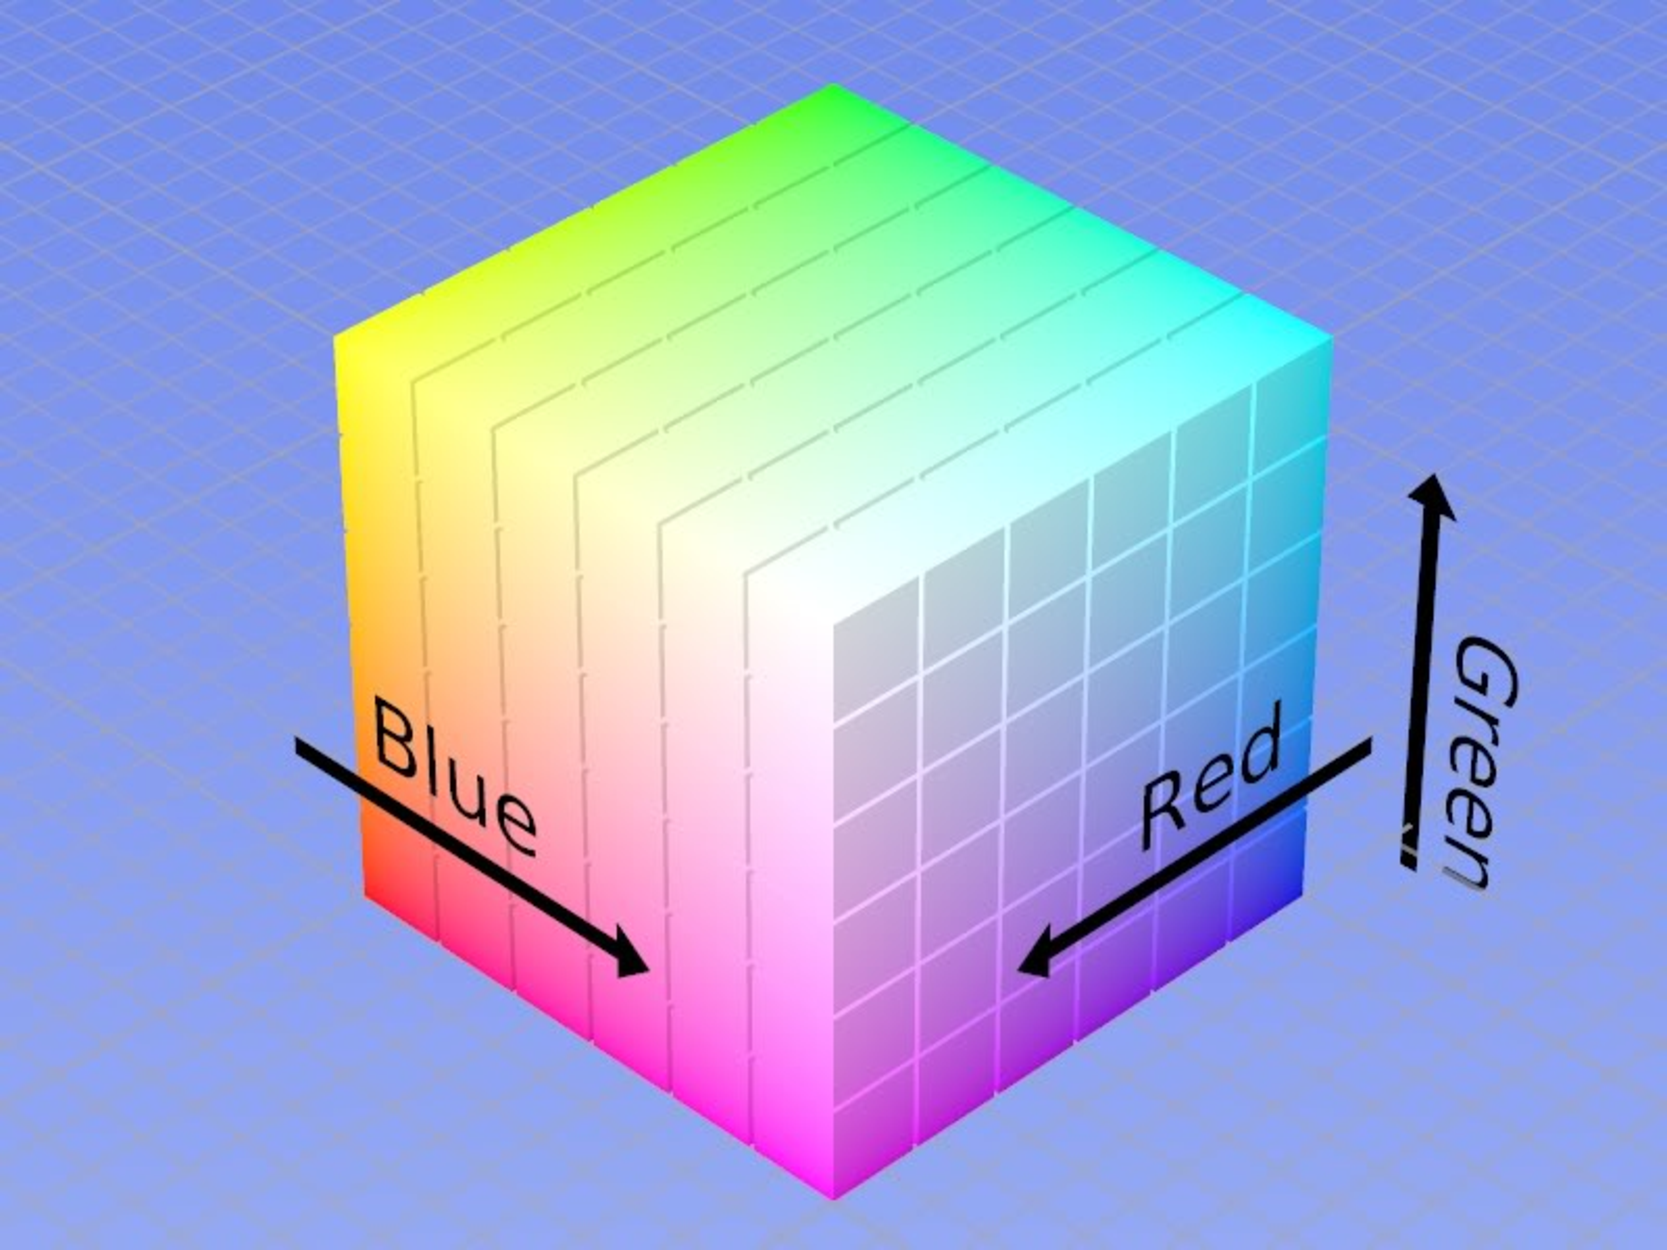
\includegraphics[width=0.4\textwidth]{rgb.pdf}
	
\caption{Exemplo do Modelo de Cor RGB.	 \citeonline{ImagensHSLHSVRGB}  }
	\label{fig:ModeloRGB}
\end{figure}

O modelo HSV, representado pela Figura \ref{fig:ModeloHSV}, é definido pela tonalidade({\it Hue}) que é a cor em si, variando de 0 a 360º; a saturação({\it Saturation}) que define o grau de pureza da cor, variando de 0 a 1; e luminância ({\it Value}) que representa os tons de ciza, que faz referência à percepção humana, também variando de 0 a 1 \cite{Leao:2005, Azevedo:2003}.
O modelo HSV utiliza definições de cor mais intuitivas que o conjunto de cores primárias, por isso são mais adequados quando se necessita obter várias tonalidades da mesma cor.

\begin{figure}[!h]
	\centering
	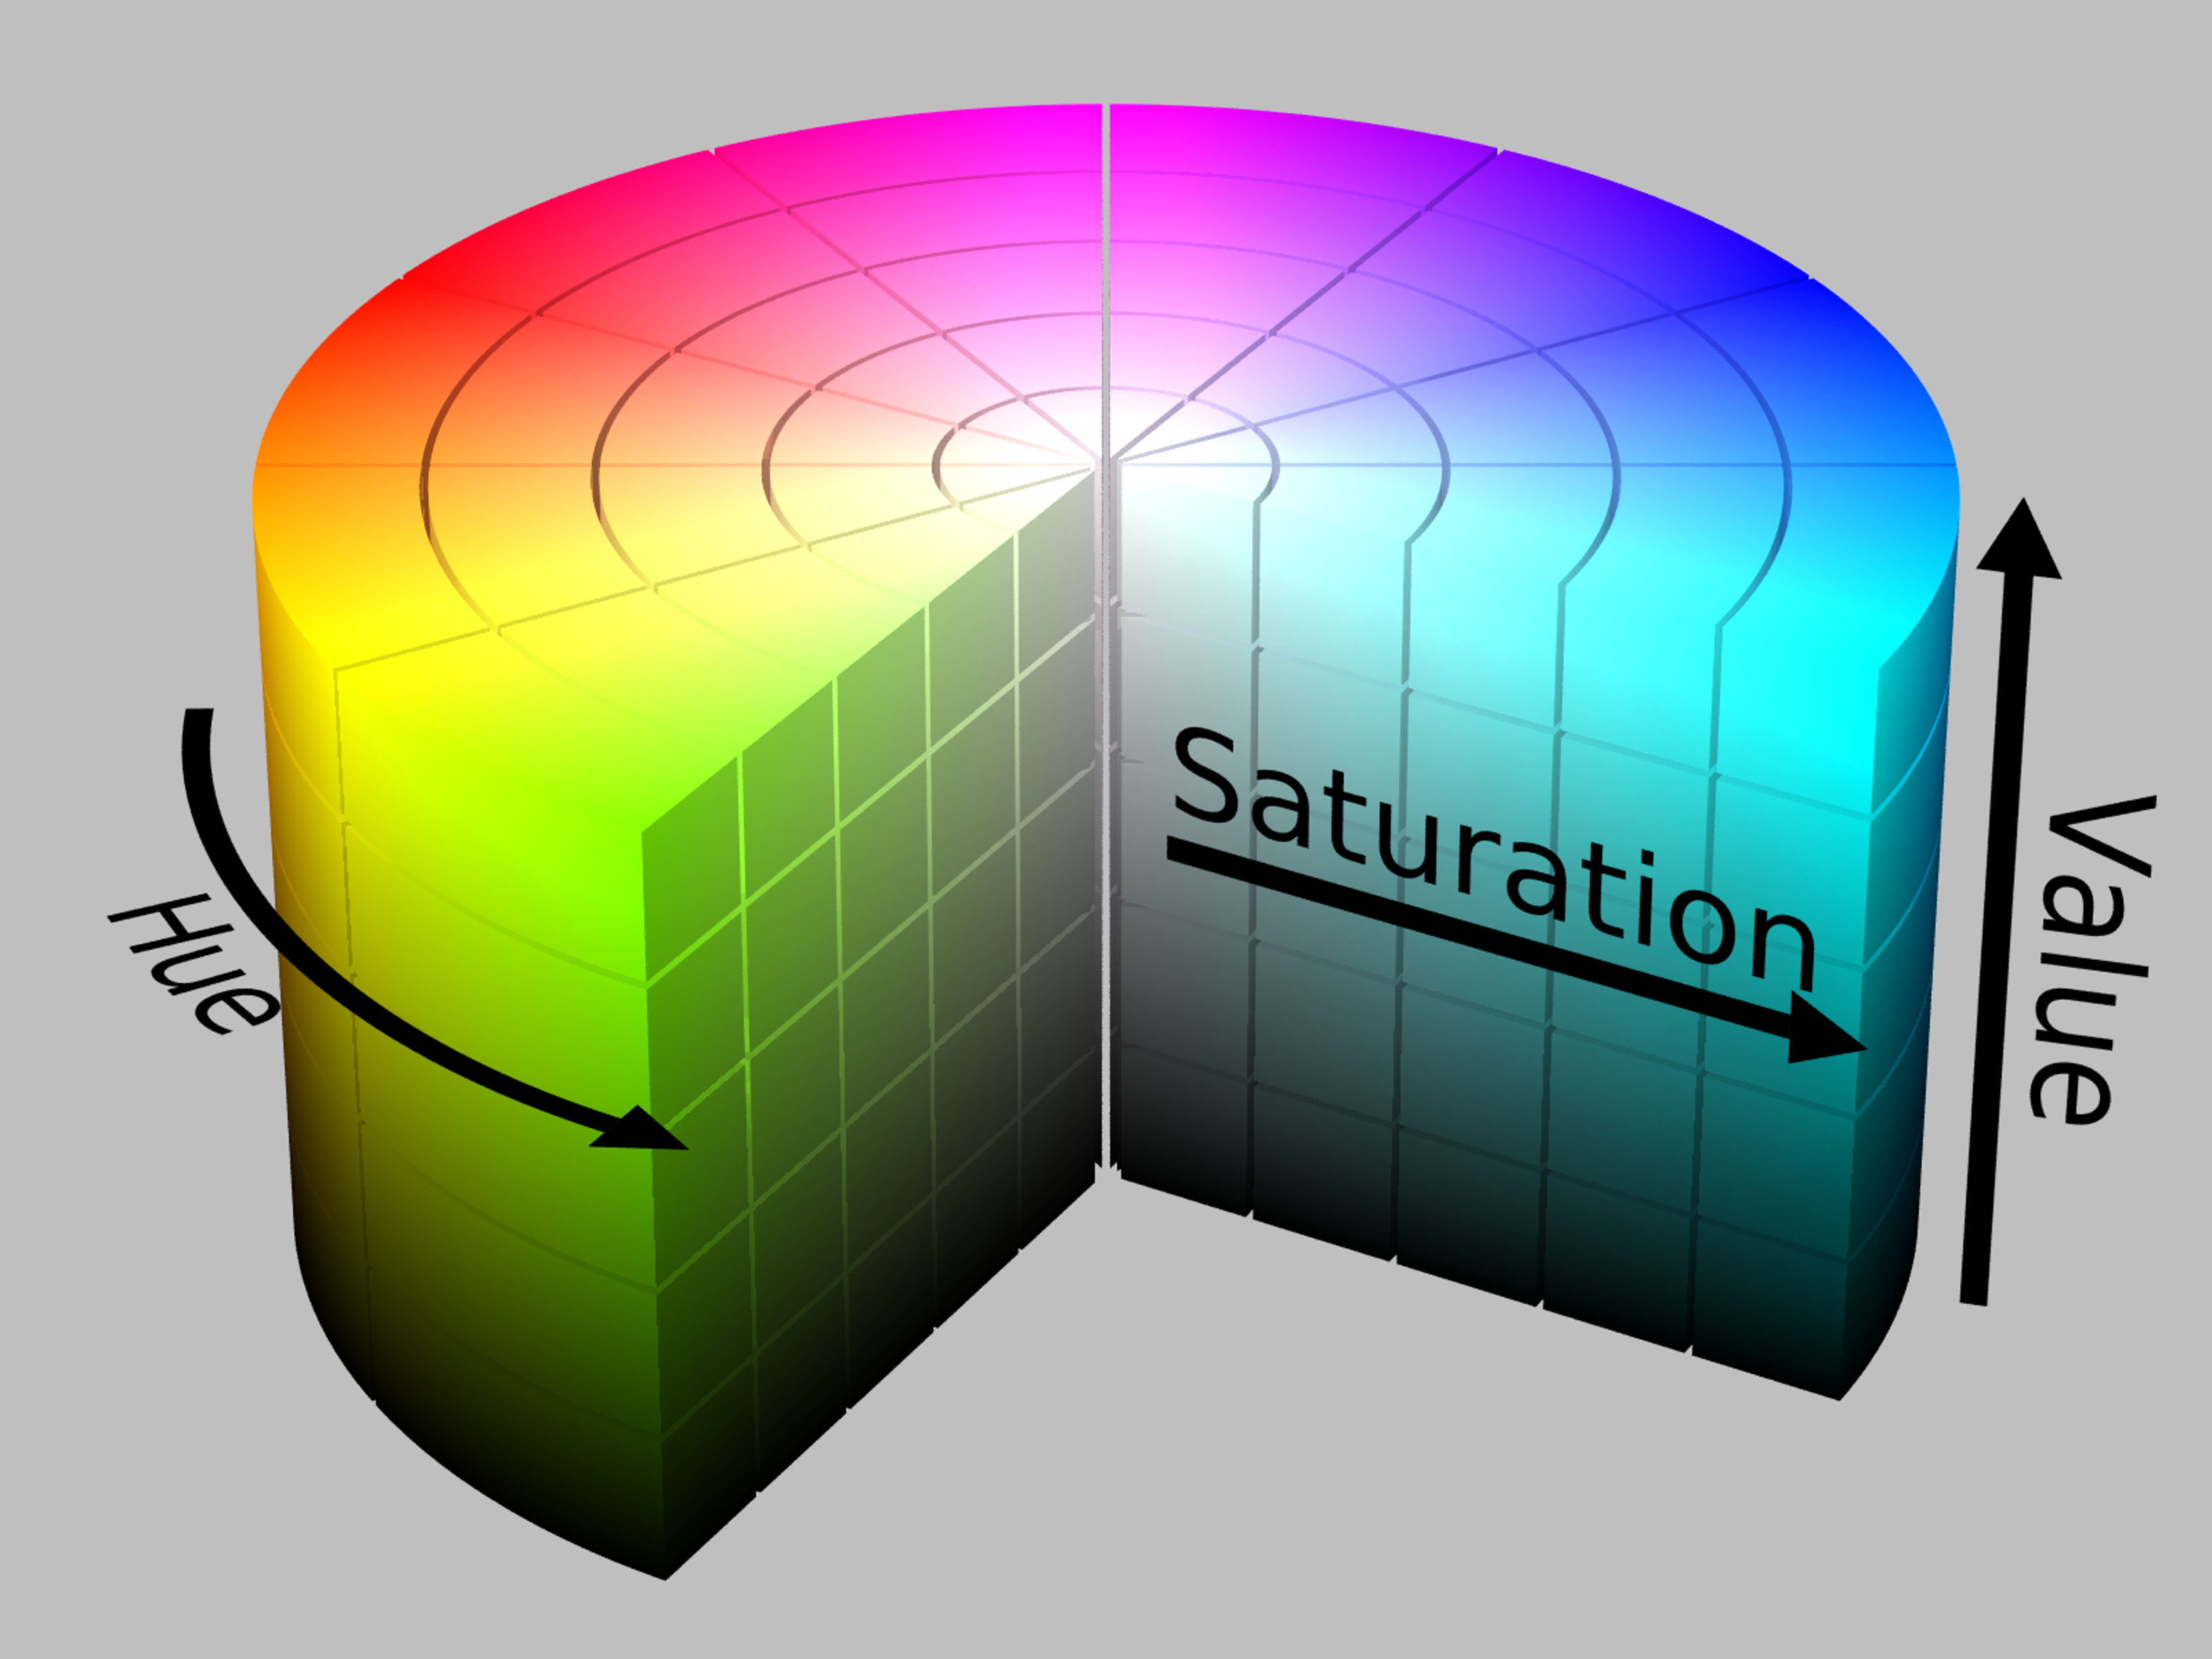
\includegraphics[width=0.4\textwidth]{hsv.pdf}
	
	\caption{Exemplo do Modelo de Cor HSV, \citeonline{ImagensHSLHSVRGB}}
	\label{fig:ModeloHSV}
\end{figure} 


\section{Futebol de Robôs}
 Visto como um domínio bastante complexo, dinâmico e imprevisível, o futebol de robôs surgiu como uma tentativa de promover pesquisas nos campos de Inteligência Artificial e robótica, pela avaliação teorias, algoritmos e arquiteturas por meio de problemas \cite{FariaIEEE2006,Costa:2000,Kitano:1997}. Além disso pode-se considerar o futebol de robôs um problema padrão, no qual se torna possível fazer a avaliação de algoritmos, arquiteturas, desempenhos e teorias \cite{Faria2006}.

 A Equipe Cedro se enquadra na categoria VSSS que é regulamentada pelo Instituto de Engenheiros Eletricistas e Eletrônicos(IEEE) e possui regras baseadas na MiroSot \cite{Tiene:2014}. O futebol de robôs se assemelha ao futebol humano cujo o objetivo do jogo é fazer gols para vencer a partida, porém tendo regras adaptadas para o âmbito robótico. \citeonline{Rosa:2015} e  \citeonline{Tiene:2014} fazem boas enumeração das regras básicas:
 \begin{itemize}
 	\item A equipe deve ser constituída por 3 robôs, sendo 1 destes o goleiro; 
 	\item Cada robô deve ter seu tamanho limita à 7,5 cm x 7,5 cm x 7,5 cm;
 \item A partida dura 10 minutos com dois tempos de 5 minutos;
  \item Há um intervalo de 10 minutos entre um tempo e outro;
   \item Cada time tem direito a dois tempos de 2 minutos que podem ser pedidos a qualquer
   momento;
   \item Durante o tempo de jogo somente são permitidas 2 substituições;
    \item Caso a diferença de gols entre os dois times chegue a 10 a partida é encerrada;
     \item Uma falta ocorre quando há mais de um robô de um mesmo time dentro de sua própria
     área de gol ou quando um robô empurrar outro robô de outro time;
     \item Um pênalti ocorre quando a bola fica mais de 10 segundos dentro de alguma das áreas;
     \item Um chute-livre ocorre quando os robôs ficam travados por mais de 10 segundos, caso
     ocorra, o juiz posiciona a bola na marca de chute-livre mais próxima de onde ela ficou
     parada e posiciona os robôs de cada time equidistantes a bola;
     \item A câmera usada pelo sistema de visão computacional deve estar acima do centro do campo, para que não seja necessário ser reposicionada quando os times trocarem de lado;
     \item A câmera deve estar à uma altura minima de 2 metros;
     \item A cada inicio de partida ou gol feito a bola deve ser posicionada no centro do campo e os
     robôs devem ser posicionados de acordo com a posse de bola.
 \end{itemize}
Uma ótima descrição do ambiente de futebol de robôs foi dada por \citeonline{Faria2006} e pode ser visualizada na Figura \ref{fig:VSSS}:
\begin{quotation}
\textit{
``(...) futebol de robôs considera-se uma câmera para capturar
a imagem de todo o campo e utilizando-se de recursos de processamento de imagem, um
computador poderá fornecer as posições dos robôs pertencentes ao time, dos adversários,
do gol e da bola. Um computador, chamado de técnico, pode utilizar algum sistema de
controle que utilize as informações disponíveis para dar ordens de como os robôs de seu
time devem agir."}\cite{Faria2006}
\end{quotation}
 \begin{figure}[H]
	\centering
	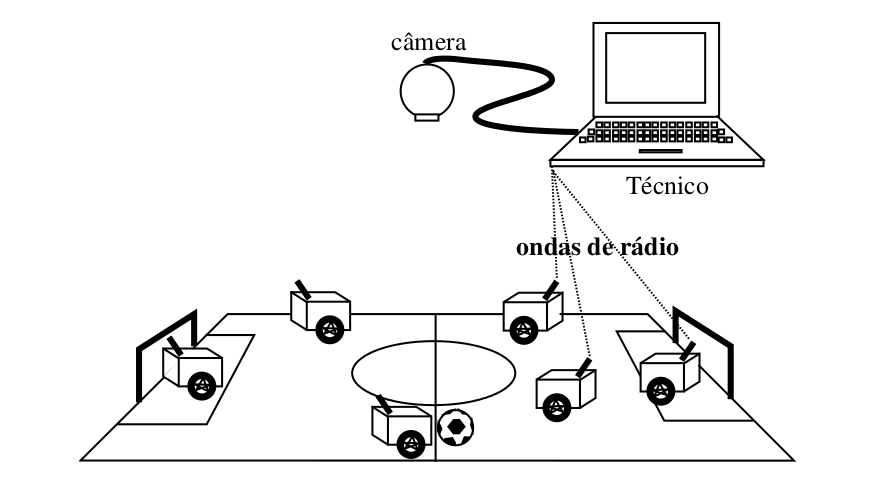
\includegraphics[width=0.4\textwidth]{faria2006.png}
	\caption{Estrutura de um ambiente de futebol de robôs VSSS\cite{Faria2006}}
	\label{fig:VSSS}
\end{figure} 
\section{Considerações Finais}